% Chapter 5

\chapter{SYSTEM DEVELOPMENT} % Write in your own chapter title

\section{Input and Output to System}
\subsection{Input}
Input to the system consists of sensor data by the IMU, JSON-encoded orientation data from the app and images taken by the RPi camera to the quadcopter.
\subsection{Output}
The output of the system consists of automatic stabilization of the quadcopter's flight, change in orientation of the quadcoper and image processing functions respectively.
\newline
1) An upward swipe on the left joystick results in increase in altitude of the quadcopter\newline
2) A downward swipe on the left joystick results in decrease in altitude of the quadcopter\newline
3) An upward swipe on the right joystick results in the quadcopter pitching forward i.e. increase in the back motors\newline
4) A downward swipe on the right joystick results in the quadcopter pitching backward i.e. increase in the front motors\newline
5) An swipe right on the right joystick results in the quadcopter pitching right i.e. increase in the left motors\newline
6) An swipe left on the right joystick results in the quadcopter pitching left i.e. increase in the right motors\newline
\section{Input and Output for each module}
\subsection{Raspberry Pi-controlled quadcopter}
\textbf{Input}\newline
The input to Raspberry Pi is the gesture packets from the internet.\newline
1. IMU sensor-data from the accelerometer and gyroscope regrading acceleration and angular velocity.\newline
2. JSON-encoded orientation data from the Android app.\newline
3. JSON-encoded image-acquisition signal data from the Android App.\newline
\textbf{Output}\newline
There are 3 kinds of outputs based on the input to the quadcopter.\newline
1. IMU sensor data is used ny the PID algorithm to calculate the required orientation and stabilize the quad automatically.\newline
2. Orientation (x,y, z) data is sent to the quad to make it move to the left/right or increase/decrease in altitude.\newline
3. Image acquisition signals allow the RPi camera to click pictures and store them.\newline
\textbf{Process}\newline
\textbf{Code for Python Server}\newline
\begin{lstlisting}
s = socket.socket()         
host = '0.0.0.0'      
port = 12345          
s.bind((host, port))   
s.listen(5)            
c, addr = s.accept()   
print 'Got connection from', addr
bus = smbus.SMBus(1)
while True:
  try:
    msg=c.recv(1024)
    data = json.loads(msg)
    if 'reset' in data:
      quadcopter.set_zero_angle()
      continue
    p = int(data['P'])
    i = int(data['I'])
    d = int(data['D'])
    height = int(data['pitch'])
    quadcopter.set_height(height)
    quadcopter.set_PID(p,i,d)
    except Exception as e:
      print e
quadcopter.stop()
c.close()        
\end{lstlisting} 
\textbf{Code for Balancing the Quad using PID}\newline
\begin{lstlisting}
while self.running:
            start_time = time.time()
            old_pitch, old_roll, old_yaw = pitch, roll, yaw
            (pitch, roll, yaw) = self.imu.read_pitch_roll_yaw()
            (_, _, gx, gy, _, ax, ay, _) = self.imu.read_all()
            axis_output = {'x': 0, 'y': 0, 'z': 0}
            [axis_output['x'],i_x]=self.compute_PID_output(self.kp_x, self.ki_x, self.kd_x, pitch-self.offset_x, i_x, old_pitch)
            [axis_output['y'],i_y]=self.compute_PID_output(self.kp_y, self.ki_y, self.kd_x, roll-self.offset_y, i_y, old_roll)
            [axis_output['z'],i_z]=self.compute_PID_output(self.kp_z, self.ki_z, self.kd_x, yaw-self.offset_z, i_z, old_yaw)
            self.motor_bl.setW(int(self.height+axis_output['x']/2
              +axis_output['y']/2))
            self.motor_br.setW(int(self.height+axis_output['x']/2
              -axis_output['y']/2))
            self.motor_fl.setW(int(self.height-axis_output['x']/2
              +axis_output['y']/2))
            self.motor_fr.setW(int(self.height-axis_output['x']/2
              -axis_output['y']/2))
            end_time = time.time()
            print end_time-start_time
            while(end_time-start_time <= 0.02):
                end_time = time.time()
                time.sleep(0.0001)
            i=i+1
\end{lstlisting} 
\subsection{Image-Processing Module}
This module is split into two parts:\newline
1. Panorama stitching\newline
2. 3D Model Reconstruction\newline
\newline
\textbf{Input - Panorama Stitching}\newline
The input consists of images taken by the RPi camera.\newline
\textbf{Output}\newline
Stitched images forming a 360 degree equirectangular panorama image.\newline
\textbf{Process}\newline
\begin{lstlisting}
  image_1 = imread(path_to_image_1)
  image_2 = imread(path_to_image_2)

  (keypoints1, descriptors1) = detect_and_compute(image_1)
  (keypoints2, descriptors2) = detect_and_compute(image_2)
  matches = knn(descriptors1,descriptors2)
  points1 = new Array(keypoints1[i] for (i,j) in matches)
  points2 = new Array(keypoints2[j] for (i,j) in matches)
  homography = find_homography(points1,points2)
  (size, offset) = calculate_size(image_1, image_2, homography)
  warped_image = warp_perspective(image_2,homography)
  panorama = warped_image
  panorama[offset_x:offset_x+image_1_width,offset_y:offset_y+image_1_height] = image_1
\end{lstlisting}
\textbf{Input - 3D Reconstruction}\newline
The input consists of images taken by the RPi camera.\newline
\textbf{Output}\newline
Sparse point-cloud representing 3D model of the images taken by the quadcopter rendered on a browser.\newline
\textbf{Process}\newline
\begin{lstlisting}
images = read_images(image_path)
for each image in images:
  features = detect_features(image)
  save_features(features)
matches = {}
for each image1 in images:
  for each image2 in images:
    if image1 not equal to image2:
      count = match_features(image1.features,image1.features)
      if count > threshold:
        matches[image1] = image2
        for each image1 in matches:
          for match in matches[image1]:
            track = add_track(image1,image2)
            create_track_graph(track)
            im1, im2 = find_images_with_largest_matches(images)
            pts3d = bootstrap_reconstruction(im1,im2)
            for each image in images:
              if image not equal to im1 and if image not equal to im2:
                pts2d = get_keypoints(im2)
                pts3d = incremental_reconstruction(pts3d,pts2d)
                pts3d = bundle_adjustment(pts3d)
\end{lstlisting}

\subsection{Android App Module}
\textbf{Input}\newline
Touch and click (Haptic) controlled movements on the virtual joystick interface of the app. \newline
\textbf{Output}\newline
Touch movement on the circular joystick results in change in orientation of the quad.
Clicking the camera button send a signal to the RPi Camera to take pictures.
\newline
\textbf{Process}\newline
Joystick Interface
\begin{lstlisting}
joystick_left = new Joystick()
joystick_right = new Joystick()
joystick_left.setTouchListener()
joystick_right.setTouchListener()
camera_button.setClickListener()

camera_button.click(){
  camera.shoot()
  camera.enable()
}

while(app_running)
{
  action_left = joystick_left.touch()
  action_right = joystick_right.touch()
  distance_left = joystick_left.getDistance()
  distance_right = joystick_right.getDistance()
  switch(action_left)
  {
    case 'up': increase_height(distance_left)
               break
    case 'down': decrease_height(distance_left)
               break
    default: print 'Invalid action'
  }
  switch(action_right)
  {
    case 'up': pitch_forward(distance_right)
               break
    case 'down': pitch_backward(distance_right)
                 break
    case 'left': pitch_left(distance_right)
                 break
    case 'right': pitch_right(distance_right)
                  break
    case 'upleft': pitch_upleft(distance_right)
                   break
    case 'upright': pitch_upright(distance_right)
                    break
    case 'downleft': pitch_downleft(distance_right)
                     break
    case 'downright': pitch_downright(distance_right)
                      break
    default: print 'Invalid action'
  }
}
\end{lstlisting}


\section{Modules}
\subsection{Raspberry Pi 2-controlled quadcopter}
The objective of the project was to build a semi-autonomous quadcopter capable of self-controlled, stable flight guided via wireless communication through an Android app. 
A quadcopter, also called a quadrotor helicopter or quadrotor, is a multirotor helicopter that is lifted and propelled by four rotors. Quadcopters differ from conventional helicopters. They use rotors which are able to vary the pitch of their blades dynamically as they move around the rotor hub. In the early days of flight, quadcopters (then referred to as 'quadrotors') were seen as possible solutions to some of the persistent problems in vertical flight; torque-induced control issues (as well as efficiency issues originating from the tail rotor, which generates no useful lift) can be eliminated by counter-rotation and the relatively short blades are much easier to construct.
The quadcopter utilises Raspberry Pi microcomputer that runs Python and takes care of all the on-board computation. It also holds an accelerometer, gyroscope, IMU sensor, GPS and a Raspberry Pi native camera.
The Raspberry Pi through python programming, interfaces with the IMU to find out the current orientation of the quadcopter and accordingly controls the motors. The IMU consists of an accelerometer, gyroscope ( and an optional magnetometer ) which accurately provides the current orientation of quadcopter including the G-force and angular velocity. The Raspberry Pi interfaces with the IMU using an I2C interface that allows it to communicate with the accelerometers, gyroscopes and magnetometers independently using only 2 pins(viz. SCL and SDA pins) by using separate addresses for each. The Pi gets the accelerometer and gyroscope angles separately for each axis and computes on them to find out the overall orientation of the quadcopter.
The Raspberry Pi can only supply digital signals that is 0 or 1 i.e. on or off. This does not allow us to directly control the motors to vary their speed. The Electronic Speed Controller ( ESC ) allows such digital signals to be converted to variable voltage and allow speed regulation of motors by supplying a PWM signal to them. PWM signals are achieved by sending pulses at a certain frequency while controlling the amount of time the pulse is on in a cycle. The longer the pulse is high during a cycle, the higher the voltage supplied to the motor. The ESC also allows an external power souce such as a battery to be used for powering the motors. Our drone uses a 10V LiPo battery. LiPo batteries are commonly used for powering drones because they have high discharge rates required to power the four motors functioning at high speed and requiring order of 20A of current. 

Write PID stuff here

The quadcopter's flight is controlled using a PID ( Proportional-Integral-Derivative ) controller.  The PID algorithm takes in the roll,pitch and yaw values fed by the IMU and calculates the required orientation values.

Write Python Server here

The quadcopter flight and on-board operations are controlled via WiFi using an Android app. JSON-encoded data is sent from the app to the python server running on the quadcopter which decodes the data and executes the required programs.
The quadcopter houses a native Pi camera module which has the ability to take high quality photos and videos. It interfaces with the Raspberry Pi using a Camera Serial Interface. 
The function of the quadcopter is to take pictures and perform two major image-processing operations viz. Panorama Stitching and 3D-Model Reconstruction.
The drone can take several images of a wide physical space. The Pi then stitches the images together using OpenCV image-processing library to construct a panorama image ( which is a wide photo obtained from multiple images ). The second operation is 3D Model reconstruction wherein, the images taken by the quadcopter can be fed to a Structure from Motion ( SfM ) algorithm to construct sparse point clouds.
The quadcopter itself is small enough to control its flight and large enough to hold all the on-board equipment.


\begin{figure}[H]
  \centering
  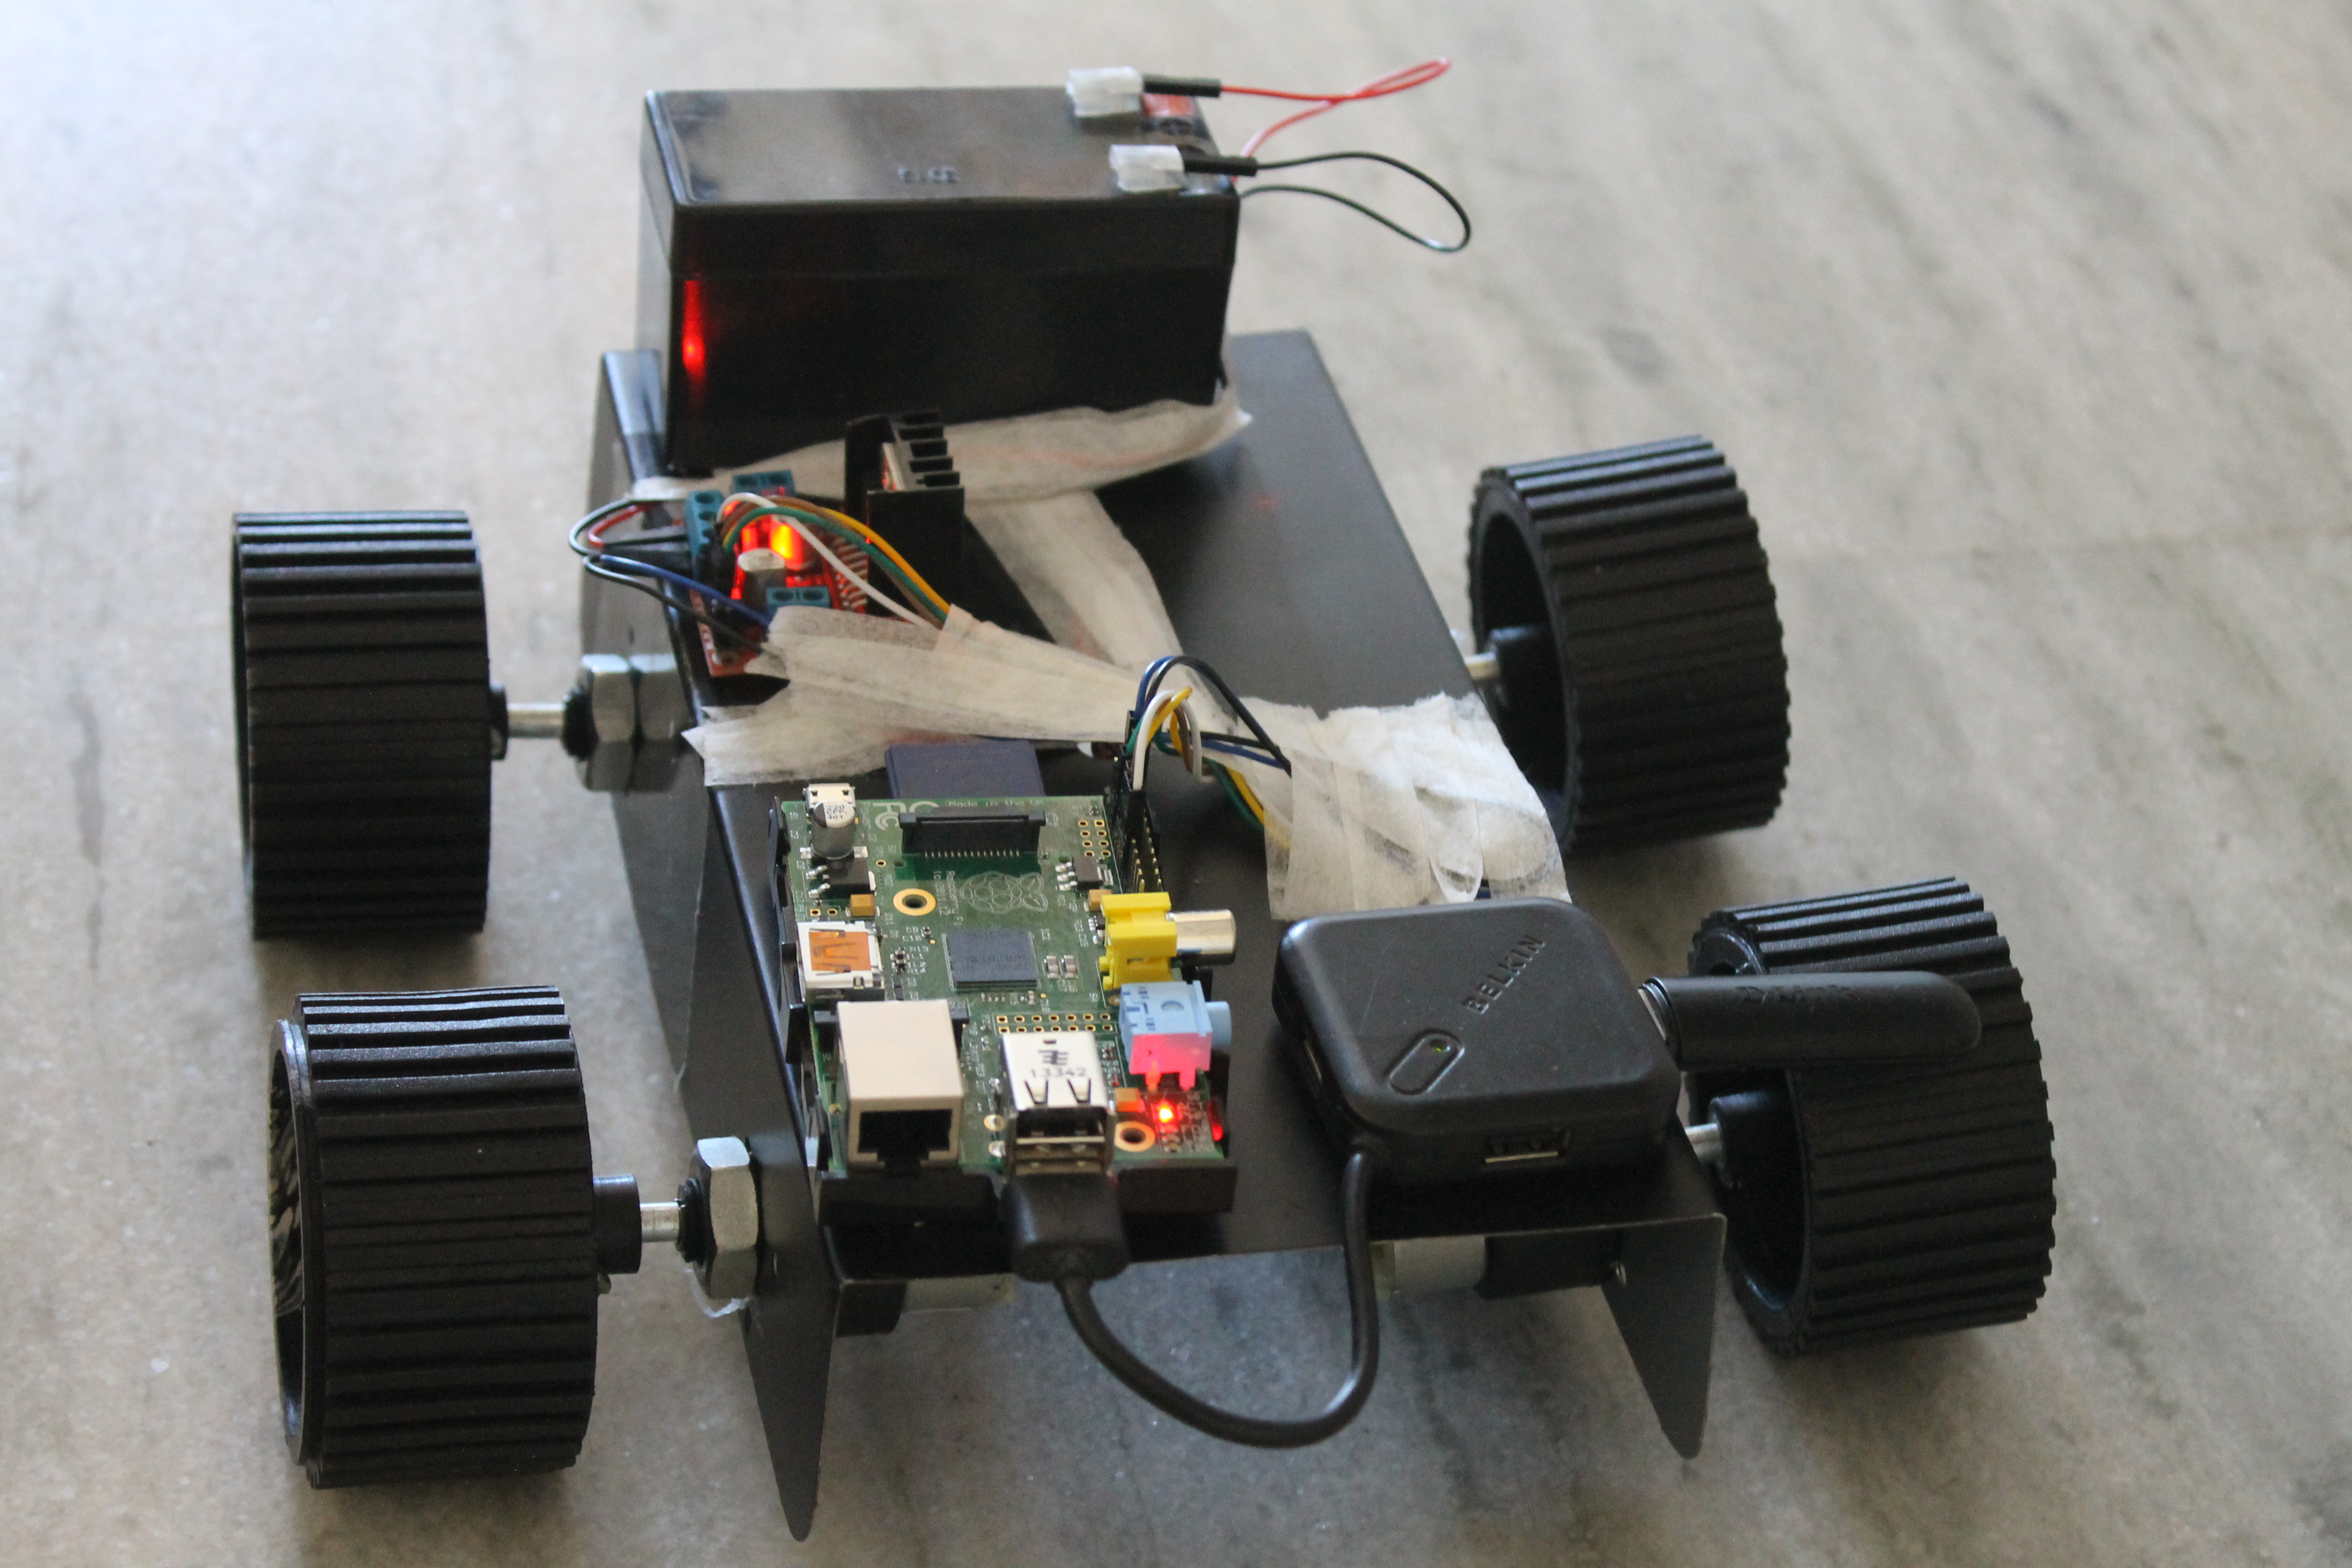
\includegraphics[width = 15cm, height = 11cm]{InitialRobot.jpg}
  \caption{The Preliminary Quadcopter without the camera}
  \label{first quadcopter}	
\end{figure}

\begin{figure}[H]
  \centering
  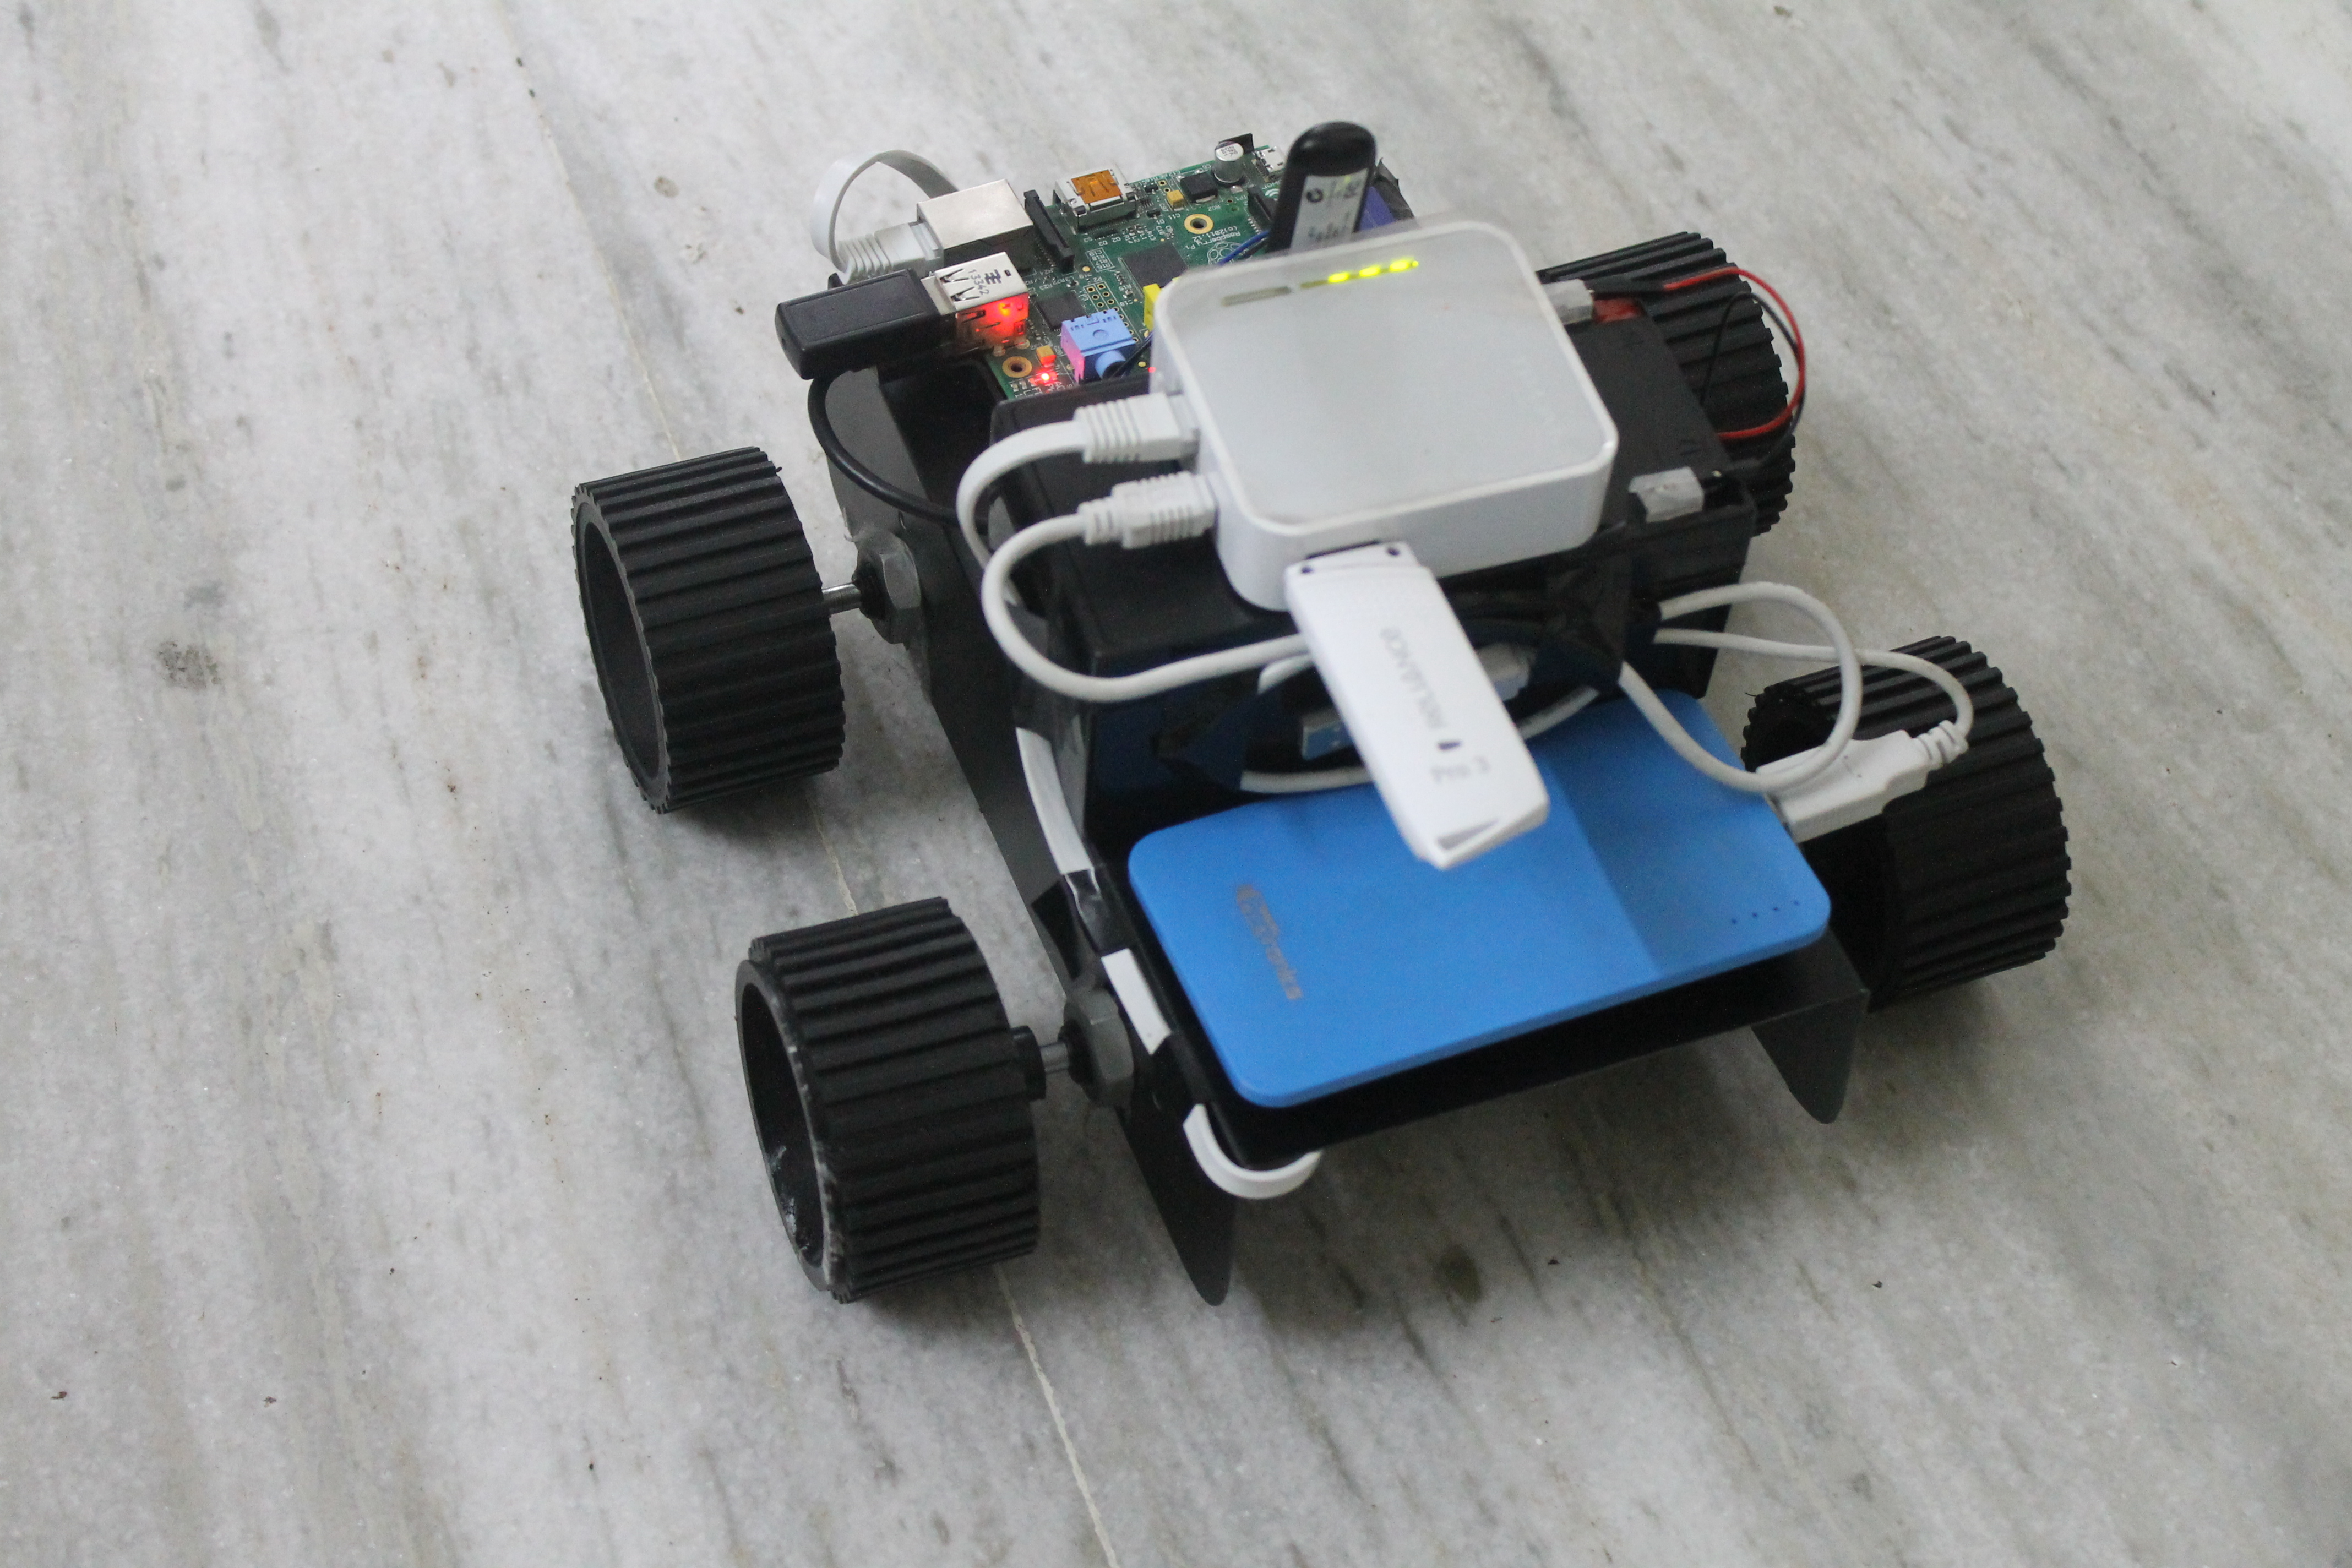
\includegraphics[width = 15cm, height = 11cm]{SecondRobot.jpg}
  \caption{The Fully Functional Quadcopter with the Camera}
  \label{second quadcopter}	
\end{figure}



\subsection{Image-Processing Module}
The objective of the project is to build a quadcopter that can perform Panorama Stitching and 3D Reconstruction of images taken during its flight. The reason we chose these functions is because the drone is mobile and can reach and capture pictures of inaccessible locations like tall buildings and surveying wide-open spaces. OpenCV is an open-source image processing library which has an enormous number of functionally-rich libraries and detailed online documentation. OpenCV  Version 3.1.0 ( the latest version ) is used to provide image-processing support in this project.
The image-processing module is divided into two parts – Stitching and Reconstruction. The initial stages are the same for both the operations i.e. Acquisition of images, Detecting Features and Matching Features.  Feature detection is accomplished using SURF ( Speeded Up Robust Features  algorithm and Feature Matching is done by building Kd-Trees and using (K-Nearest Neighbours) Flann Algorithm.
For Panorama Stitching, after feature-matching, RANSAC ( Random Sample Consensus ) is used to detect outliers and construct a homography matrix. The Homography matrix is then used to warp the images and construct a panorama. The stitching process is quite fast for fewer images but in order to speed up the process for a large number of images, we have implemented a multi-threaded stitching algorithm that stitches images in parallel, thereby, reducing the time without compromising on the quality(distortion) of the panorama generated.
 3D-Recontruction is implemented by using Structure from Motion(SfM) algorithm. The preliminary stage is to calibrate the Pi Camera and calculate intrinsic and extrinsic camera paramaters. Once camera calibration is complete, the images have to be preprocessed to collect metadata i.e. EXIF tags which hold important GPS, latitude, longitude and camera information. The next stages are the feature detection and matching stages which have been described above. Matching features are then collected into tracks and a graph of these good “tracks” is constructed. The next stage is to use the graph to find common tracks and construct the 3D point cloud in incrementally. Initially, two images with a large number of matches are chosen for the “bootstrap reconstruction”. The reconstruction consists of triangulating the 2D points to 3D points which can be visualized as a point cloud. Consequently, the rest of the images' points are added incrementally to the point cloud. After each addition, “Bundle Adjustment” is done to minimize the reprojection error. This is the most computationally-intensive step. Once all the images have been added to the reconstruction, the final point cloud is generated and stored as a “.ply” file. The Point Cloud is visualized in an interactive browser environment using a Javascript Library called, “threeJS” on a remote system.   

\begin{figure}[H]
  \centering
  \includegraphics[width = 15cm, height = 12cm]{SkeletalRecognition.jpg}
  \caption{Panorama Stitching of test images}
  \label{pano}	
\end{figure}

\begin{figure}[H]
  \centering
  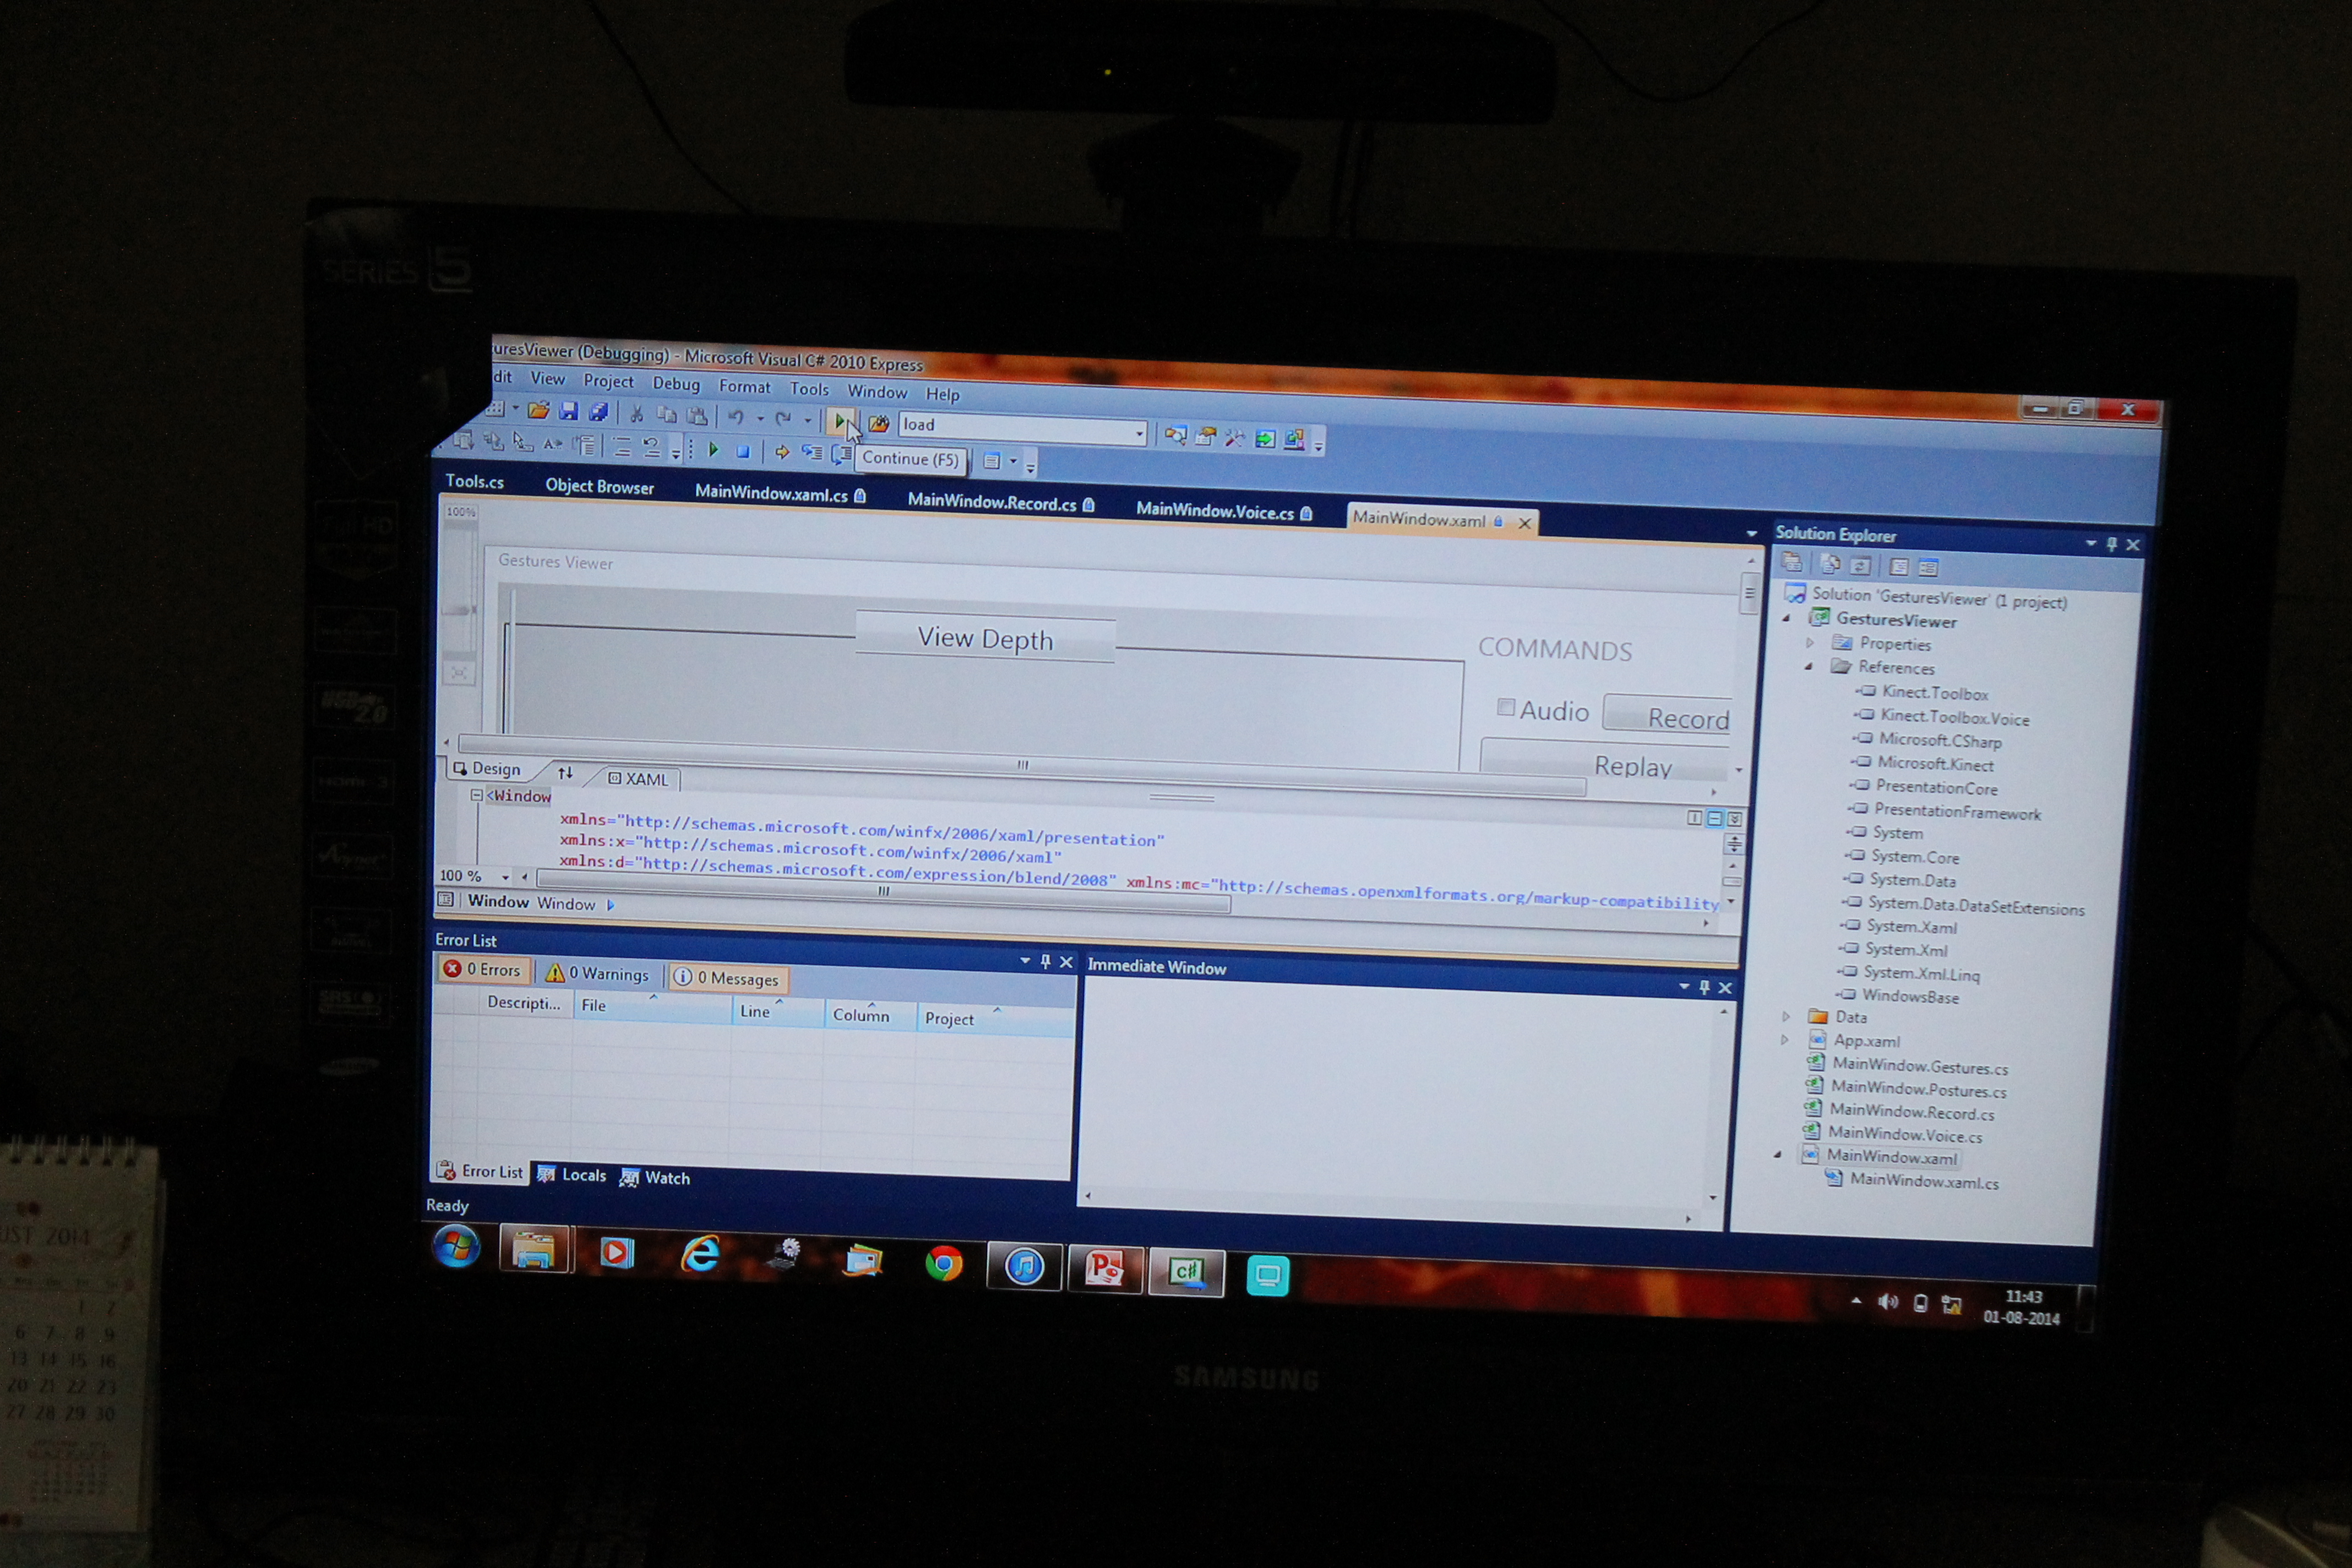
\includegraphics[width = 15cm, height = 12cm]{WPF.jpg}
  \caption{3D Reconstruction of test images}
  \label{recon}	
\end{figure}

\subsection{Android App}
Todo

\section{Software Implementation Flow}

\begin{figure}[H]
  \centering
  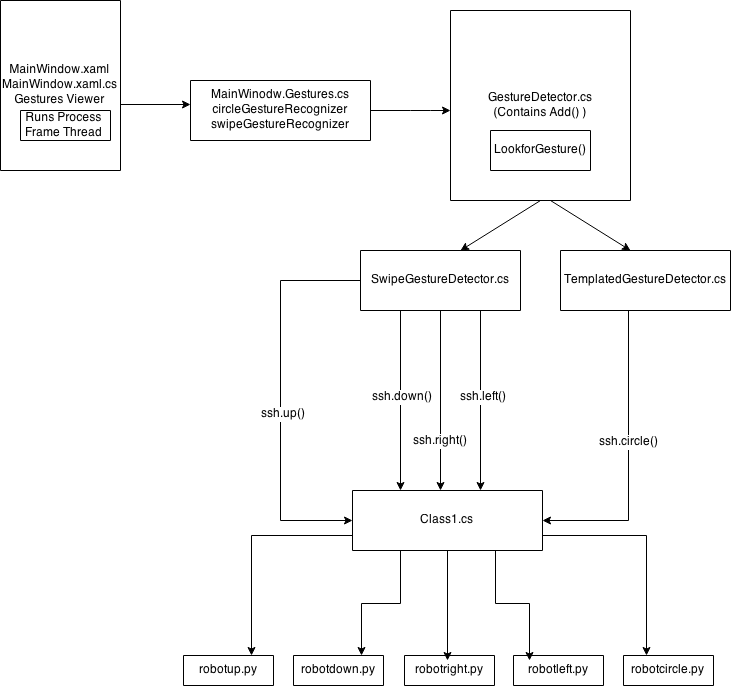
\includegraphics[width = 15cm, height = 12cm]{software.png}
  \caption{Software Flow Diagram}
  \label{Software Flow}	
\end{figure}

